\chapter{Implementing a Parser for \Beluga}\label{chapter:parsing-reimplementation}

This chapter presents an overview of parsing and explains the motivation behind the contributions made to \Beluga's and \Harpoon's parsing algorithms.
Some aspects of context-sensitive disambiguation of \acp{AST} are showcased, including grammars for parsing user-defined prefix, infix and postfix operators.

\section{Introduction}\label{section:parser-introduction}

This section provides a conceptual introduction to parsing, a discussion on the concept of ambiguity in parsing, and finally an overview of concepts and features of parsers for programming languages in proof assistants.
Notably, we motivate the introduction of semantic analysis as part of syntactic analysis when it comes to resolving ambiguities in a language like \Beluga.

% What is parsing?

In compiler design, parsing is the process of converting the textual representation of a program into a hierarchical data structure~\cite{aho2007compilers, afroozeh2019practical}, which is typically called a parse tree.
When a parse tree captures all the data about the text being processed, including comments and parentheses, then it is referred to as a concrete syntax tree.
Otherwise, when parts of the data have been abstracted away, it is instead called an \ac{AST}.

% What is ambiguity in parsing?

A program's textual representation is ambiguous with respect to a predefined set of parse rules if the program can be parsed into a parse forest, which is multiple parse trees~\cite{aho2007compilers}.
By way of analogy, a sentence in a natural language is ambiguous if it can be interpreted in multiple valid ways with respect to its syntactic and grammatical rules.
Since programming languages are tools for describing computerized systems, it is necessary that each valid written program has exactly one interpretation~\cite{aho2007compilers}.
In the strictest of cases, this unicity of interpretation may be enforced at the level of the grammar and parser, such that all syntactically valid programs have exactly one inferable interpretation.
This is typically achieved using rules and syntactic conventions that prevent ambiguous programs from being ever written in the first place.

Certain kinds of syntactic ambiguities are unavoidable in programming languages, and are frequently useful to the end user.
Indeed, programming languages often reuse or overload syntactic constructs to reduce both the number and the complexity of rules that users have to learn in order to read and write programs.
Ambiguous syntax can also make programs more terse, which may improve some workflows~\cite{resolveAmbiguity}.
Additional mechanisms need to be put in place as part of the compiler's implementation to detect syntactic ambiguities, and either signal them as errors, or resolve them using additional interpretation rules.

% What is disambiguation in parsing?

Disambiguation is the process by which a parse forest is filtered down to a single parse tree.
It refers to the procedures used to resolve ambiguities in intermediate results of parsing.
In parsing systems that do not output parse forests, disambiguation typically involves manipulating the \ac{AST} representation of a single parse tree that captures ambiguities, meaning that some of its nodes represent the overlapping of syntactic constructs.
Functionally, these nodes suspend parsing until more information is available to disambiguate them to the correct node variant.

% What is the impact of disambiguation on program readability?

Increasing the amount of computation required to disambiguate the textual representation of a program negatively impacts the maintainability and readability of that program for the end user.
Indeed, some forms of ambiguity in the syntax of a program may prevent the end user from fully understanding it in isolation from the rest of the code sections.
As such, one can argue that the programmatic strategies for disambiguating the syntax of a programming language should be intuitive so that external software is not required for the end user to read a program.
For instance, name resolution is sufficiently intuitive for users, whereas searching in a parse forest for a parse tree that type-checks is not necessarily intuitive, especially given the complexity of some type systems.
Hence, trade-offs between functionality and ease of understanding must be made when designing a language.

% What are some examples of syntactic ambiguities?

Different kinds of concrete syntax ambiguities may arise during parsing of a programming language.
We distinguish three kinds of syntactic ambiguities that come into play in the implementation of \Beluga, listed below in increasing degree of cognitive complexity required to solve them:
\begin{enumerate}
\item
\textit{Static operator ambiguities}: operators and their operands may be interpreted in different orders depending on where they appear in a whitespace-delimited list of terms.
For instance, the expression $a + b * c$ is ambiguous with respect to the grammar $e\coloneqq e+e\mid e*e$.
These ambiguities are typically resolved by assigning a precedence level, a fixity and an associativity to each operator in the language, and parsing them as keywords.
\item
\textit{Name-based ambiguities}: overloaded identifiers may be resolved to different binding sites depending on where they appear in an expression, and fall under different semantic categories as a consequence.
For instance, in a dependently-typed language, type-level and term-level variables may be syntactically ambiguous, but they may have distinct syntaxes for binders.
Semantic analysis of the \ac{AST} with respect to a symbol table is usually sufficient to disambiguate those cases.
However, overloading of identifiers coupled with more advanced features, like user-defined mixfix operators~\cite{danielsson2008parsing}, poses additional challenges since identifiers may not be considered in isolation.
\item
\textit{Type-based ambiguities}: the correct interpretation of an expression may only be determined once a type has been inferred for it, or if it is checked against a type.
This does not refer to method overloading in object-oriented programming languages since the syntax for calling a method is not ambiguous.
Rather, if the expression being parsed is an identifier, then a type-based ambiguity may be that that expression or a surrounding one falls into a different syntactic category based on the identifier's type or kind.
For instance, the syntax $ \texttt{(g, x : t)} $ may denote a pair of terms, with the variable $ \texttt{x} $ being checked against the type $ \texttt{t} $, or it may denote the context $ \texttt{g} $ with an added variable declaration $ \texttt{x : t} $.
In this case, what $ \texttt{(g, x : t)} $ syntactically denotes depends on the type of $ \texttt{g} $.
To solve such ambiguities, some type information may be provided by a symbol table if the type ascribed to an identifier is known at the declaration site.
In general it is not practical to disambiguate expressions having type-based ambiguities before type-checking, especially when more intricate type inference algorithms need to be applied to determine the type of an identifier.
Because of this, languages are typically designed to avoid type-based ambiguities.
In the same way that is done in figure~\ref{figure:internal-syntax}, identifiers like $\psi$ can be reserved to always denote contexts, such that $\texttt{($\psi$, x : t)}$ is unambiguously a context.
\end{enumerate}

% What do ambiguities have to do with language design?
% What is the typical workflow for designing syntaxes and implementing parsers? What are parser generators? What are their limitations?

The kinds of syntactic ambiguities that arise in the design of a programming language depend on the system used to specify its syntax, which in turn affects the algorithm required to parse it.
The concrete syntax of programming languages is typically specified with a \ac{CFG}, denoted in \ac{EBNF}.
If a language can be specified by a \ac{CFG}, then it is a \ac{CFL}.
\Acp{CFL} have many advantages, including the fact that there is an abundance of well-vetted parser generators for such languages.
\ocamllex together with \ocamlyacc~\cite{smith2007ocamllex} is one example of such a parser generator.
Crucially, \acp{CFL} are easy to parse, both algorithmically and by the end user.
As the name suggests, parsers for \acp{CFL} does not require additional data in a context specifically intended for disambiguation.
This ensures that programs can scale and be readable by the user without having to fully know the context in which programs appear.
That is, other code sections in a \ac{CFL} do not affect how a given code section is parsed.
Static operator ambiguities as mentioned previously can be resolved by rewriting the grammar while keeping it context-free.
Name-based and type-based ambiguities however give rise to context-sensitive languages, or even strictly Turing-recognizable languages~\cite{chomsky1956three}.
Context-sensitive languages necessitate additional data about the context in which parts of a program appear to correctly parse it.
This typically means that some semantic analysis is required during parsing in order to complete the syntactic analysis.
Consequently, the concrete syntax's design for a programming language is intrinsically linked with the algorithm required to parse it.

% What are some language design considerations?

We say that a grammar is dynamic (or user-extensible, or featuring syntax extensions) if the way a program is parsed is influenced by directives in the program itself, and otherwise we say that the grammar is static.
Languages for specifying logics tend to favour user-extensible grammars over static ones.
Indeed, \Agda and \Isabelle/\HOL support mixfix operators, \Coq has notation declarations, and \Beluga, like \Twelf, has prefix, infix and postfix operators specified by pragmas.
This is justified by the need for more concise and expressive ways to convey the meaning of definitions and lemmas.
Such syntax extensions also allow users to develop mechanizations with notations that are closer to what appears on pen-and-paper proofs.
However, that design choice negatively impacts the implementation of external tools for the language.
Indeed, user-defined syntax extensions complicate the implementation of incremental parsing for efficiently parsing edits in a text editor, as well as indexing for resolving identifiers to their binding site.
This forces tooling to be tightly coupled with the core implementation of the language.
%This is notably the case for tooling in \Cpp because of its rich pre-processor that increases the complexity of parsing and name resolution.

Early versions of the \Beluga language were context-free and used \CamlpFour~\cite{de2003camlp4} as parser generator to implement its parser.
\Beluga became context-sensitive when modifications were made to its syntax, specifically to improve the readability of contextual objects and to add user-defined operators as in \Twelf for \LF type-level and term-level constants.
These changes did not pose a problem with the parser's implementation per se, but it did require the introduction of disambiguation mechanisms, or rather the inclusion of syntactically ambiguous nodes in the signature reconstruction algorithm.
Specifically, parts of indexing and reconstruction, as illustrated in figure~\ref{figure:legacy-beluga-processing-pipeline}, and the elaboration steps in between, had to be implemented with \ac{AST} node variants that mix together syntactically ambiguous constructs.
This complicated the processing pipeline since the semantics of a given \Beluga program is only gradually discovered as it is elaborated through the external, approximate and internal syntax representations.
%The data-dependent semantic rules necessary to complete the syntactic analysis are hence difficult to convey to end users.

% What are parser combinators? What are some well-known libraries for parser combinators? What are their limitations?

As the \Beluga language grew, so did the complexity of its grammar, such that user errors output by the parser generated with \CamlpFour were deemed not sufficiently informative.
Hence, \Beluga version \texttt{1.0} featured a new parser implemented using monadic parser combinators, which are higher-order functions for constructing top-down recursive descent parsers~\cite{Burge1975-BURRPT, hutton1996monadic, leijen2001parsec, generalparsercombs, afroozeh2019practical}.
They provide a more declarative way of constructing complex parsers than shift-reduce parsers.
Indeed, the combination of smaller parsers (or parselets) in \OCaml using operators closely resembles grammar specifications using \acp{CFG}, which allows for fast prototyping and better readability of the implementation.
As such, the intent of reworking \Beluga to use parser combinators was to improve error-reporting for the end user, and to improve the overall maintainability of the implementation for subsequent developers by making it more modular.
These objectives were largely met, and as a consequence \Harpoon was also implemented using that parsing framework.
%However, one may argue that shifting from a parser generator implementation to parser combinators was detrimental to the system's maintainability since that discarded the benefits of static analyses of the language's grammar for ambiguities.
There is still room to improve in the way of user-friendly error messages to help newcomers get a better grasp of the language and its features.
As discussed in the following sections, these shortcomings in error reporting are partly due to the extensive use of overlapping syntactic constructs.
However, the more significant contributing factor is the stringent syntactic restrictions influenced by the internal workings of the processing pipeline.
%This also applies to both the internal and user-facing documentation of \Beluga's syntax.

\clearpage

\section{\Beluga Lexing, Parsing and Disambiguation Phases}\label{section:lexing-parsing-disambiguation}

As part of this thesis, \Beluga's parser was reimplemented to handle expressions in non-canonical form, to support user-defined operators at the level of computations, and to improve the implementation's maintainability.
Particularly, semantic analysis is introduced as part of a new context-sensitive disambiguation phase to the parser in order to produce a fully unambiguous \ac{AST} before signature reconstruction.
The motivation for these changes to the implementation of \Beluga can be summarized in the following points:
\begin{enumerate}
\item
\textit{Expand the operator pragmas feature to computation-level types and expressions.}
By implementing a reusable process for disambiguating function applications, any juxtaposition of terms in the language's grammar can feature user-defined operators.
\item
\textit{Improve syntax error messages.}
By accepting a wider range of programs during parsing, the subsequent disambiguation phase can more precisely identify the cause for syntax errors and report them with better detail.
\item
\textit{Improve the processing pipeline's maintainability.}
By decoupling disambiguation from indexing, both phases now respect the single-responsibility principle, which in turn simplifies the information flow at the early stage of signature reconstruction.
Dependency injection of mutable states is also introduced define clear boundaries on effects in the implementation of the disambiguation phase, which enables the development of structured editing procedures.
\item
\textit{Provide unambiguous external \acp{AST} to enable debugging of signature reconstruction.}
Since the disambiguated external \ac{AST} of a program fully captures the meaning of what the user wrote, then the internal \ac{AST} as illustrated in figure~\ref{figure:legacy-beluga-processing-pipeline} is no longer the only unambiguous data representation for programs in \Beluga.
This clear boundary in the system allows for isolated testing of the parser, and provides a point of comparison with the internal syntax \ac{AST} output from signature reconstruction.
\end{enumerate}

A complete specification of \Beluga's and \Harpoon's syntax is provided in appendix~\ref{chapter:grammar} to facilitate future changes to the language, and to provide documentation to the end user.
The revised parsing algorithm for \Beluga signatures is split into three phases, namely: lexing, parsing and disambiguation.
These phases are outlined in the next subsections.
First, lexing is implemented just like in typical whitespace-agnostic programming languages, except for one lexer hack used to handle some overloading of a static operator.
Then, parsing produces an \ac{AST} close to the concrete syntax and featuring ambiguous nodes, which effectively postpones parsing steps that require external data.
Finally, disambiguation converts the parsed \ac{AST} to a revised external \ac{AST} without ambiguous nodes.

\subsection{Lexing}

Lexical analysis for \Beluga uses regular expressions to convert sequences of characters into tokens to speed up recursive descent parsing.
Appendixes~\ref{section:comments-lexical-convention}, \ref{section:keywords-lexical-convention} and \ref{section:lexical-convention} provide the functional requirements for this phase of the implementation.
Notably, lexing of nested delimited comments (i.e., those comments enclosed in either \verb|%{| and \verb|}%|, or \verb|%{{| and \verb|}}%|) is achieved by parameterizing the comment-lexing function with respect to the depth of the comment.
This ensures that extraneous or missing right-delimiters for comments are detected early.

Where the lexing phase diverges from conventional implementations is with regards to its dot operator.
Indeed, usual lexical conventions dictate that whitespace may precede or follow a dot without affecting a program's semantics.
This cannot apply unambiguously in \Beluga programs, where a dot denotes one the following:
\begin{enumerate}
\item
The end of an \LF term-level or type-level constant declaration, like in \Twelf.
\item
The beginning of a computation-level observation application for coinductive objects.
\item
The delimiter between the parameter name and the body of an \LF $\lambda$-abstraction.
\item
The projection out of a contextual \LF block term.
\item
The projection out of a computation-level tuple expression.
\item
The projection out of a module acting as a namespace.
\end{enumerate}

This first usage of the dot operator proved particularly difficult to resolve when the operator was overloaded with projections out of namespaces.
One approach to solve this issue is to use a different operator for accessing members of modules, which deviates from how \textsc{ML}-style languages are designed.
The solution that was ultimately put in place was to instead introduce two additional token kinds \synt{dot-identifier} and \synt{dot-integer} in the lexer for identifiers and numbers immediately prefixed by a dot.
These token kinds were reserved to denote projections.
During context-free parsing, wherever a dot is expected to not be part of a projection, these two token kinds would still be accepted, but a corresponding identifier or number token would be spliced in the input stream.
This effectively means that whitespace cannot follow a dot operator used for projection.
Thus, \Twelf-style \LF term-level and type-level constant declarations could be parsed in \Beluga, provided that the trailing dot is followed by whitespace.

This token insertion solution had to be introduced to preserve backward compatibility in the parser, specifically for that \Twelf-style of constant declarations.
In general, it is inadvisable to mutate the stream of tokens during parsing, especially in the presence of unbounded backtracking since those insertions may have to be reverted.

\subsection{Parsing}

Parsing of \Beluga signatures is achieved using $ \mathsf{LL(\infty)} $ parsing in pathological cases and $ \mathsf{LL(1)} $ parsing in the most frequent cases.
This is implemented using the monadic parser combinator library introduced in \Beluga version \texttt{1.0}.
Unlimited lookahead is enabled only in select cases, or if no input token has been consumed, which performs efficiently enough for large \Beluga files.

The main contribution made to the context-free parsing phase of \Beluga is the simplification of its grammar.
Indeed, the legacy parser was designed following the grammars developed along signature reconstruction and type-checking algorithms, which introduced syntactic classes that ensure some properties always hold by construction for terms in the language.
Specifically, the index level \LF of \Beluga is strongly-normalizing, and \LF terms in canonical form cannot feature certain kinds of non-termination in term reduction, then it was decided that the user should only be able to write \LF terms and types in canonical form.
This required that nonterminals be introduced for normal and neutral terms separately to mirror the syntax of figure~\ref{figure:internal-syntax}.
Additionally, since \Beluga's type-checking algorithm is bidirectional, computation-level expressions were split into two syntactic classes, namely type-synthesizing expressions and type-checkable expressions, and this change was also reflected in the parser.
Implementation efforts revealed however that these syntactic constraints are too stringent to be imposed during parsing.
Indeed, they increased the complexity of the parser, made operator precedence rules opaque, and yielded poor syntax error messages to the user.
This is because the pre-terms of \Beluga cannot be elegantly partitioned all at once by order of precedence, by whether they are neutral or normal, and by whether they synthesize a type or check against one.
This partitioning is required for recursive descent parsing, but those parser rules are too complex to be explained to newcomers to the language, and are also error-prone for developers.
The additional constraints further restrict the language recognized by the parser, which in turn prevents some syntactically invalid programs from being reported with more precision than simply identifying unexpected tokens.
This is in part evidenced by the grammar in figure~\ref{figure:legacy-clf-parsing} and the example syntax error message in figure~\ref{figure:improved-syntax-error-message}.
As such, the revised parser's grammar does not distinguish between neutral and normal terms, nor type-synthesizing and type-checkable expressions.
This greatly broadens the scope of programs accepted by the parser, which in turn allows for later phases of processing to report and reject non-canonical terms with greater flexibility for error-reporting.

\begin{figure}[H]
\begin{grammar}
<clf-normal> ::=
     `\\' <identifier> `.' <clf-term-application>
\alt `(' <clf-term-application> [`:' <clf-type>] `)'
\alt <hash-identifier> [<clf-projection>] [ `[' <clf-substitution> `]' ]
\alt <qualified-identifier> [<clf-projection>] [ `[' <clf-substitution> `]' ]
\alt `_'
\alt `?'<identifier>
\alt `<' <clf-term-application> (`;' <clf-term-application>)+ `>'

<clf-projection> ::=
     `.' <integer>
\alt `.' <identifier>

<clf-term-application> ::=
     <clf-normal>+
\alt <clf-type>

<clf-type> ::=
     `{' <identifier> `:' <clf-type> `}' [`->'] <clf-type>
\alt <clf-type-atomic> [`->' <clf-type>]

<clf-type-atomic> ::=
     <clf-normal>+
\alt <identifier> <clf-normal>*
\alt `(' <clf-type> `)'
\alt `block' `(' <identifier> `:' <clf-type> (`,' <identifier> `:' <clf-type>)+ `)'
\end{grammar}
\caption[The grammar for parsing contextual \acs{LF} terms in normal form in the legacy \Beluga parser]{%
The grammar based on figure~\ref{figure:internal-syntax} for parsing contextual \LF terms in normal form in the legacy parser, denoted using the lexical conventions of section~\ref{section:lexical-convention}.
The definition for the nonterminal \synt{clf-substitution} is omitted for brevity.
The nonterminals \synt{clf-term-application} and \synt{clf-type-atomic} showcase a dramatic increase in complexity for parsing contextual \LF terms and types.
This presentation also does not effectively demonstrate that left recursions never occur, and what precedence each operator has.
}
\label{figure:legacy-clf-parsing}
\end{figure}

\begin{figure}[H]
\begin{subfigure}{\linewidth}
\begin{Verbatim}[commandchars=\\\{\}, baselinestretch=1]
exp : \verbbf{type}.
eq : exp -> exp -> \verbbf{type}.
\verbbf{schema} ctx = \verbbf{block} (x : exp, t : eq x x);
\verbbf{rec} reflexivity : \{g : ctx\} \{M : [g |- exp]\} [g |- (eq M M)[..]] = ?;
\end{Verbatim}
\caption{%
Example \Beluga theorem statement with a syntactically invalid substitution.
The identity substitution \texttt{[..]} on the application of an \LF type constant in \texttt{(eq M M)[..]} is invalid because only canonical forms of \LF objects are recognized for signature reconstruction.
}
\end{subfigure}
\par\bigskip
\begin{subfigure}{\linewidth}
\begin{Verbatim}[baselinestretch=1]
example.bel, line 5, column 59:
Parse error.
Unexpected token in stream
  Expected token `]'
  Got token `['
\end{Verbatim}
\caption{%
The syntax error raised during context-free parsing in the legacy parser implementation.
Given the stricter grammar of \synt{clf-type} in figure~\ref{figure:legacy-clf-parsing}, it is true that the token \texttt{[} introducing the identity substitution is unexpected.
However, the reason for this error is not obvious from its message, in part because the user unambiguously wrote a substitution.
}
\end{subfigure}
\par\bigskip
\begin{subfigure}{\linewidth}
\begin{Verbatim}[commandchars=\\\{\}, baselinestretch=1]
\verbpbf{File "example.bel", line 5, column 52:}
5 |rec reflexivity : \{g : ctx\} \{M : [g |- exp]\} [g |- (eq M M)[..]] = ?;
                                                      \verbrbf{^^^^^^^^^^^^}
\verbrbf{Error:} Substitution terms may not appear as contextual LF types.
\end{Verbatim}
\caption{%
Improved syntax error message produced during the disambiguation phase instead of during context-free parsing.
Using a relaxed grammar for \LF objects to support non-canonical forms, the parser accepts the invalid substitution, and then the disambiguation phase identifies that it should be rejected.
}
\end{subfigure}
\caption[Example of improved syntax error reporting]{%
Example of improved syntax error reporting using less stringent syntactic rules at the level of the parser.
}
\label{figure:improved-syntax-error-message}
\end{figure}

\clearpage

Besides the aforementioned simplifications to the grammar, the revised parser still has to support the syntax of \LF kinds, types and terms, which overloads operators.
For instance, the $\to$ operator is overloaded for arrow kinds and types, and the syntaxes for $\Pi$-kinds and $\Pi$-types are the same in \Beluga.
This means that an \LF kind is syntactically indistinguishable from an \LF type until a $\mathbf{type}$ kind is encountered as the very last operand since \LF kinds necessarily contain one.
Unrestricted backtracking and infinite lookaheads are not suitable solutions to this disambiguation issue given that those expressions are the most frequent ones in \Beluga signatures.

The implemented solution to this sort of problem during context-free parsing is somewhat counterintuitive.
The syntactic categories having common syntaxes that appear in ambiguous positions are merged into a single nonterminal in the grammar.
We call this blurring the grammar since we effectively lose the distinction between those merged syntactic categories during context-free parsing.
This results in a grammar that accepts a wider range of expressions.
Hence, an additional phase of processing is required to recover a parser for the initial grammars.
Section~\ref{section:blurred-lf-syntax} provides an example of one such blurred grammar, obtained by merging the nonterminals \synt{lf-kind}, \synt{lf-type} and \synt{lf-term} of section~\ref{section:syntax-lf} into one syntactic category, with corresponding nonterminal \synt{lf-object}.
The context-sensitive disambiguation phase outlined in the next section is then tasked with recovering the original \LF kind, type or term corresponding to a parsed \LF object.
We note that a similar technique was used in \Twelf since its shift-reduce parser could not perform disambiguation during parsing.

\subsection{Disambiguation}

The disambiguation phase of parsing performs an \ac{AST} transformation from the parser syntax to the external syntax.
Given \Beluga's features and overloaded syntactic constructs, disambiguation is responsible for recovering the structure specified by the grammars of section~\ref{section:syntax} using the structure obtained by context-free parsing following the blurred grammars of section~\ref{section:resolving-grammar-ambiguities}.
Specifically, it performs disambiguation of:
\begin{enumerate}
\item \LF kinds, types and terms,
\item contextual \LF types and terms,
\item meta-level contexts and substitutions,
\item computation-level kinds and types, and
\item applications throughout the semantic classes (detailed in section~\ref{section:parsing-user-defined-operators}).
\end{enumerate}

Disambiguation of \Beluga programs requires that identifiers be resolved to their binding sites in order to determine their sort.
This process statefully keeps track of the identifiers in scope at any given point during a traversal of the parser \ac{AST}.
This environment is implemented using a mutable state structure with auxiliary data to deal with patterns, modules and pragmas.
Specifically, bindings during this phase are modelled using a stack of scopes, each of which contains a tree mapping fully qualified identifiers to minimal descriptions of what those identifiers are bound to (namely variables or constants).
In particular, the referencing environment records the user-defined notation to use for any given identifier.
This allows for fixity pragmas like in figure~\ref{figure:operator-pragmas} to be declared in namespaces, and to later be brought in scope when the namespace is opened.
Additionally, notations can be locally redefined since the referencing environment defines the area of effect for those pragmas.
Then, applications in the concrete syntax, which were parsed as lists of terms, can be reparsed in a context-sensitive manner during disambiguation.

We postpone the discussion on how the referencing environment is constructed and updated during the \ac{AST} traversal to section~\ref{section:indexing} because it closely follows the procedure used to compute de Bruijn indices during the indexing phase.

\section{Parsing User-Defined Operators}\label{section:parsing-user-defined-operators}

In \Beluga, users may specify that identifiers should be used as operators in expression applications, as shown in figure~\ref{figure:operator-pragmas}, using \verb|--prefix|, \verb|--infix| or \verb|--postfix| pragmas.
Prefix operators are unary and right-associative, postfix operators are unary and left-associative, and infix operators are binary and may be either left-associative, right-associative or non-associative.
The priority of operations is specified using integer precedence values.
This feature was ported over from \Twelf, and using the new parsing architecture, it was subsequently improved to support shadowing of operators by bound variables and other constants.
As outlined below, the notation pragmas for user-defined operators in \Beluga are more restrictive than that of \Agda because \Beluga does not support mixfix operators~\cite{danielsson2008parsing}.

\begin{figure}[htb]
\begin{Verbatim}[commandchars=\\\{\}, baselinestretch=1, numbers=left]
\verbbf{LF} p : \verbbf{type} =
| \makebox[1em]{⊃} : p \makebox[1em]{→} p \makebox[1em]{→} p                  \verbcomment{% Logical implication}
| \makebox[1em]{⊂} : p \makebox[1em]{→} p \makebox[1em]{→} p                  \verbcomment{% Converse implication}
| \makebox[1em]{∧} : p \makebox[1em]{→} p \makebox[1em]{→} p                  \verbcomment{% Logical conjunction}
| \makebox[1em]{∨} : p \makebox[1em]{→} p \makebox[1em]{→} p                  \verbcomment{% Logical disjunction}
| \makebox[1em]{¬} : p \makebox[1em]{→} p                       \verbcomment{% Logical negation}
| \makebox[1em]{⊤} : p                            \verbcomment{% Tautology}
| \makebox[1em]{⊥} : p                            \verbcomment{% Contradiction}
;
\verbprag{--infix \makebox[1em]{⊃} 3 right.}    \verbcomment{% Subsequently treat ⊃ as a right-associative}
\verbprag{--infix \makebox[1em]{⊂} 3 left.}     \verbcomment{% infix operator with precedence value 3}
\verbprag{--infix \makebox[1em]{∧} 5 right.}
\verbprag{--infix \makebox[1em]{∨} 4 right.}
\verbprag{--prefix \makebox[1em]{¬} 10.}

\verbbf{let} a = [x : p \makebox[1em]{⊢} ¬ ¬ ¬ x];
\verbbf{let} b = [x : p, y : p \makebox[1em]{⊢} ¬ x ⊂ y ⊂ ⊥];
\verbbf{let} c = [x : p, y : p, z : p \makebox[1em]{⊢} ⊤ ∨ x ∧ ¬ y ⊃ ¬ z];
\verbbf{let} d = [f : p \makebox[1em]{→} p, x : p \makebox[1em]{⊢} ¬ f x ∨ f ⊥];
\end{Verbatim}
\caption[Example of user-defined operator definitions in \Beluga using pragmas]{%
Example of user-defined operator definitions in \Beluga using pragmas.
The subsequent meta-objects \texttt{a}, \texttt{b}, \texttt{c} and \texttt{d} use those notations to construct formulas just like in proofs on paper.
}
\label{figure:operator-pragmas}
\end{figure}

\begin{figure}[htb]
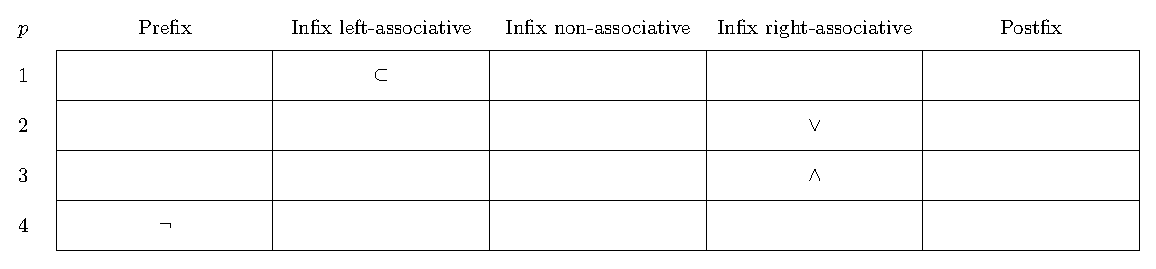
\includegraphics[width=\textwidth]{figures/operator-table.eps}
\caption[Example operator table for parsing user-defined operators]{%
Example operator table for parsing user-defined operators for applications containing only the operators $\lnot$, $\land$, $\lor$ and $\subset$ as defined in figure~\ref{figure:operator-pragmas}.
The rows are arranged in order of relative precedence for those operators.
This table would be used to parse $x \subset x \lor y \lor \lnot z \land w$ as $x \subset (x \lor (y \lor ((\lnot z) \land w)))$.
}
\label{figure:operator-table}
\end{figure}

The legacy \Beluga system only supported user-defined operators for \LF type-level and term-level applications.
As such, only constants in \LF could be defined as operators.
The implemented revisions allow for user-defined operators to be used in all applications, meaning that computation-level types and expressions may also benefit from prefix, infix and postfix notations.
Specifically, all typed constants can now be annotated with a notation pragma.
Type annotations are required in this case since disambiguation does not perform type inference.
This in turn allows for early error detection for mismatches between the arity expected by the notation pragma and the actual arity of the constant.
Using a lookahead mechanism during disambiguation, notation pragmas can be declared before their targets are in scope.
As such, their application is postponed until the constants they affect are introduced in scope.

The new implementation for parsing user-defined operators relies on the disambiguation phase for resolving identifiers to constants and their notations.
As such, the initial parser suspends parsing of applications, meaning that it represents the juxtaposition of parsemes as lists.
Disambiguation then resumes parsing with a recursive descent parser instantiated specifically for the operators that appear in the list of parsemes.
That is, when disambiguating an application node, not all constant declarations in scope at that point in the \Beluga signature need to be taken into account.
We only need to build an operator table as in figure~\ref{figure:operator-table} for the constants appearing in the application and resolved as operators in the referencing environment.
This ensures that the complexity of this second phase of parsing for applications scales only with the number of parsemes in the list, and not with the size of the signature.
However, this design requires that operators cannot be overloaded, otherwise disambiguation of applications could only be realized when type information is available, which happens much later in signature reconstruction for \Beluga.

In \Beluga, at the precedence level of expression applications, there are four scenarios to disambiguate:
\begin{enumerate}
\item Prefix operators followed by their operands,
\item Left-associative, right-associative or non-associative infix operators preceded and followed by their operands,
\item Postfix operators preceded by their operands, and
\item Juxtaposed expressions having no operator.
\end{enumerate}

During the disambiguation phase of parsing, we only need to determine the syntactic structure of applicands and arguments for parsemes in lists.
The implementation of this parsing algorithm is inspired by the general purpose expression parser from the \texttt{Parsec} library~\cite{leijen2001parsec}, as well as the parser scheme in figure~\ref{figure:user-defined-operators-grammar}, which is adapted from the parser scheme for parsing mixfix operators in~\cite{danielsson2008parsing}.
This parsing algorithm proceeds in the following steps:
\begin{enumerate}
\item Identify the constants with user-defined operator notations in the list of parsemes.
\item Group those identifiers by precedence, then by fixity and associativity, like in the table in figure~\ref{figure:operator-table}.
\item Construct a parselet for each precedence level in the operator table, such that the precedence climb delegates parsing to the parselet for the next precedence level, in increasing order.
\item Run the parselet handling the least precedence level on the list of parsemes.
\end{enumerate}
This is effectively the same principle as recursive descent parsing for a set of operators statically defined by the language's grammar, but instead implemented over a dynamic set of operators.
This set is constructed using only those constants found in the \ac{AST} node for application.
As such, this parsing algorithm for user-defined operators has $ O(n^3) $ runtime complexity, where $ n $ is the length of the list of parsemes.
Figures~\ref{figure:user-defined-operators-initial-grammar}, \ref{figure:user-defined-operators-initial-grammar-scheme} and \ref{figure:user-defined-operators-final-grammar-scheme} progressively show how to obtain an $\mathsf{LL}(1)$ grammar scheme to parse user-defined operators.
In \Beluga \texttt{v1.1}, the parser is implemented following this last grammar scheme, and using monadic parser combinators just like in the context-free parsing phase.

Coincidentally, the grammar scheme of figure~\ref{figure:user-defined-operators-initial-grammar-scheme} was used to reintroduce support for infix left and right arrow operators $\rightarrow$ and $\leftarrow$ in \LF types.
Support for the $\leftarrow$ operator had been dropped during the rewrite of the parser from \textsf{Camlp4} to monadic parser combinators.
This was due in all likelihood because of the difficulty with amending the grammar of figure~\ref{figure:legacy-clf-parsing} while respecting the precedence and associativity of operators.
As illustrated in figure~\ref{figure:user-defined-operators-grammar}, the key takeaway from reintroducing that static operator is that at a given precedence level, we can either have the application of a non-associative operator, successive applications of right-associative operators, or applications of left-associative operators.
Those three categories of operators cannot mix at the same precedence level without introducing an unresolvable ambiguity.
As such, the recursive descent parselet for $\rightarrow$ and $\leftarrow$ operators only allows one or the other operator to appear.

\begin{figure}[H]
\begin{subfigure}{\linewidth}
\centering
\begin{tabular}{rrl}
$ \angled{e} $ & $ \Coloneqq $ & $ \angled{\prefix} \; \angled{e} $\\
& $ \mid $ & $ \angled{e} \; \angled{\infix} \; \angled{e} $\\
& $ \mid $ & $ \angled{e} \; \angled{\postfix} $\\
& $ \mid $ & $ \mathbf{a}+ $
\end{tabular}
\caption{Ambiguous grammar for parsing user-defined operators. The terminal $ \mathbf{a} $ stands for expressions that were already parsed at a higher precedence level than any user-defined operator during the context-free parsing phase.
For instance, $ \mathbf{a} $ can stand for variables and projections.}
\label{figure:user-defined-operators-initial-grammar}
\end{subfigure}
\par\bigskip
\begin{subfigure}{\linewidth}
\centering
\begin{tabular}{rrl}
$ \angled{e} $ & $ \Coloneqq $ & $ \angled{e}_1 $\\
$ \angled{e}_p $ & $ \Coloneqq $ & $ \angled{e}_{p + 1} \; \angled{\infixn}_p \; \angled{e}_{p + 1} $\\
& $ \mid $ & $ \left(\angled{\prefix}_p \mid \angled{e}_{p + 1} \; \angled{\infixr}_p\right)\hspace{-0.3em}{+} \; \angled{e}_{p + 1} $\\
& $ \mid $ & $ \angled{e}_{p + 1} \; \left(\angled{\postfix}_p \mid \angled{\infixl}_p \; \angled{e}_{p + 1}\right)\hspace{-0.3em}{+} $\\
& $ \mid $ & $ \angled{e}_{p + 1} $\\
$ \angled{e}_{P + 1} $ & $ \Coloneqq $ & $ \mathbf{a}+ $
\end{tabular}
\caption{%
Initial grammar scheme for parsing user-defined operators.
$ P $ is the number of distinct precedence levels induced by the user-defined operators appearing in the application, and $ \angled{e}_p $ is the nonterminal for an expression at precedence level $ p $.
Similarly, $ \angled{\infixn}_p $, $ \angled{\infixr}_p $ and $ \angled{\infixl}_p $ stand for infix non-associative, right-associative, and left-associative operators respectively, all at precedence level $ p $.
}
\label{figure:user-defined-operators-initial-grammar-scheme}
\end{subfigure}
\caption[Grammars for parsing user-defined operators in \Beluga]{Grammars for parsing user-defined operators in \Beluga.}
\label{figure:user-defined-operators-grammar}
\end{figure}%
\begin{figure}\ContinuedFloat
\begin{subfigure}{\linewidth}
\centering
\begin{tabular}{rrl}
$ \angled{e} $ & $ \Coloneqq $ & $ \angled{e}_1 $\\
$ \angled{e}_p $ & $ \Coloneqq $ & $ \angled{\prefix}_p \; \angled{e_\text{R}}_p $\\
& $ \mid $ & $ \angled{e}_{p + 1} \; \angled{e_\text{T}}_p $\\
$ \angled{e_\text{T}}_p $ & $ \Coloneqq $ & $ \angled{\infixn}_p \; \angled{e}_{p + 1} $\\
& $ \mid $ & $ \angled{\infixr}_p \; \angled{e_\text{R}}_p $\\
& $ \mid $ & $ \angled{\infixl}_p \; \angled{e}_{p + 1} \; \angled{e_\text{L}}_p $\\
& $ \mid $ & $ \angled{\postfix}_p \; \angled{e_\text{L}}_p $\\
& $ \mid $ & $ \varepsilon $\\
$ \angled{e_\text{L}}_p $ & $ \Coloneqq $ & $ \angled{\postfix}_p \angled{e_\text{L}}_p $\\
& $ \mid $ & $ \angled{\infixl}_p \angled{e}_{p + 1} \angled{e_\text{L}}_p $\\
& $ \mid $ & $ \varepsilon $\\
$ \angled{e_\text{R}}_p $ & $ \Coloneqq $ & $ \angled{\prefix}_p \angled{e_\text{R}}_p $\\
& $ \mid $ & $ \angled{e}_{p + 1} \angled{e_\text{R}'}_p $\\
$ \angled{e_\text{R}'}_p $ & $ \Coloneqq $ & $ \angled{\infixr}_p \angled{e_\text{R}}_p $\\
& $ \mid $ & $ \varepsilon $\\
$ \angled{e}_{P + 1} $ & $ \Coloneqq $ & $ \mathbf{a}+ $
\end{tabular}
\caption{Factored grammar scheme derived from figure~\ref{figure:user-defined-operators-initial-grammar-scheme} for parsing user-defined operators.
\Beluga's parser additionally has failure productions interspersed to peek at the next token in the input stream and raise an exception if that token is an operator in an ambiguous position.}
\label{figure:user-defined-operators-final-grammar-scheme}
\end{subfigure}
\caption[]{Grammars for parsing user-defined operators in \Beluga (cont.).}
\end{figure}

\section{Discussion}

Despite the bugfixes and new features, the revised parser architecture is not without its flaws.
The additional requirement that parsing must produce an unambiguous \ac{AST} without resorting to complex disambiguation mechanisms prevents the overloading of some syntax.
In particular, meta-objects and meta-types for substitutions now have to be prefixed by \texttt{\$} to distinguish them from plain meta-objects and meta-types respectively.
For the same reason, parameter meta-types have to be prefixed by \texttt{\#}.
Furthermore, overloading of identifiers had to be discarded so that user-defined operators in applications may be disambiguated using only a lookup table.
Those breaking changes to the syntax could have been avoided had further semantic analysis been introduced during the disambiguation phase, namely to perform type-driven disambiguation.
Should \Beluga be extended to support multiple context variables in contexts, then this may be required.
Likewise, should mixfix notations be a planned feature, then identifier overloading may need to be reintroduced with type-driven disambiguation since those notations typically require the reuse of names across different operators.

Additionally, further blurring of the grammars in section~\ref{section:resolving-grammar-ambiguities} would be required to ensure that the context-free parsing phase does not have to perform infinite lookaheads.
Indeed, there is a pathological case in parsing computation-level kinds and types where an unbounded lookahead is required because of an overlapping syntax between meta-level types and computation-level types.
The performance impact of this lookahead has not been measured, but it appears to be negligible based on the performance of running the entire processing pipeline on the numerous examples that are part of the system's test suite.
Nonetheless, the observation that additional grammar blurring is required to get from an $ \mathsf{LL}(\infty) $ parser to an $ \mathsf{LL}(1) $ parser for \Beluga begs the question whether there should only be one encompassing non-terminal in the grammar of section~\ref{section:resolving-grammar-ambiguities}.
This would make the language's grammar uniform, and allow for more flexibility in overloading syntactic constructs.
However, since a parselet is required per precedence level in recursive descent parsing, and most static operators in \Beluga have distinct precedences, the resulting increase in the recursion depth for parsing could deteriorate the runtime performance of the parser.
Arguably, such a design presents more opportunities to improve the precision of syntax error messages during disambiguation.
